\section{Realizzazione}

\subsection{Divisione dei compiti}

La realizzazione del progetto è stata così suddivisa tra i membri del gruppo:
\begin{itemize}
    \item Cazzaro Michele:
        \begin{itemize}
            \item Interfaccia di registrazione e login (pagine "Registrati", "Login", "Logout");
            \item Definizione della tabella Utenti e stesura iniziale del DB;
            \item Creazione del layout flex per gestire il menu comprimibile su tablet;
            \item Stesura dei contenuti di: "Home", "Chi Siamo", "Come Raggiungerci";
            \item Definizione di un file con metodi di utility (utils.php);
            \item Aggiunte per la navigazione accessibile (Skip nav e Scroll top);
            \item Contributo alla relazione;
        \end{itemize}
    \item Contin Riccardo:
        \begin{itemize}
            \item Impostazione iniziale menù, breadcrumb e "Home";
            \item Definizione e popolamento delle tabelle "Piste" e "Impianti" del DB;
            \item Pagine HTML/PHP: "Il nostro comprensorio", "Mappa delle piste", "Dashboard Admin", "Modifica Comprensorio";
            \item PHP: dbRicky.php;
            \item JS: modificaComprensorio.js e js per la mappa;
            \item CSS: lavorato su style.css, print.css e mobile.css;
            \item Scrittura della relazione.
        \end{itemize}
    \item Speranzon Leonardo:
        \begin{itemize}
            \item Piccole modifiche al DB: tabelle Carrello, Ordini e SkipassOrdinati;
            \item Pagine HTML/PHP: "Shop", "Carrello", "Modifica Prezzi Skipass";
            \item JS: shop.js per la gestione della form dello shop;
            \item CSS: creato print.css e adattato style.css a IE10;
            \item Contributo alla relazione
        \end{itemize}
\end{itemize}

\subsection{Struttura}
    Per la struttura è stato utilizzato HTML5, rispettando sempre la sintassi XML.
    All'interno dei file .html sono presenti dei placeholder del tipo \verb|['NomePlaceholder']| che vengono sostituiti dal php per inserire elementi ripetitivi tra le varie pagine o creati dinamicamente.
    Alcuni esempi di placeholder possono essere:
    \begin{itemize}
        \item \verb|['Imports']| viene sostituito dai vari link ai fogli di stile con le relative media query ed dallo script per il funzionamento del menu;
        \item \verb|['Menu']| viene sostituito da un menu costruito dinamicamente in base alla pagina corrente e dai privilegi dell'utente;
        \item \verb|['BtnSkip']| e \verb|['BtnScroll']| vengono sostituiti dai bottoni per agevolare la navigazione del sito.
    \end{itemize}
    Tutti i file HTML sono stati inseriti all'interno della cartella html.

\subsection{Presentazione}
Lo stile, realizzato tramite fogli di stile CSS3, è fluido e scalabile per ogni tipo di schermo.
Per questo sono stati realizzati 3 diversi CSS per gli schermi: uno stile base (per i desktop), uno aggiuntivo per i tablet ed uno per gli smartphone;
la maggiore differenza nell'uso da dispositivi diversi è il menu che varia forma e voci per adattarsi al meglio.

È stato creato anche un foglio di stile specifico per la stampa delle pagine.

\subsubsection{Desktop}
Da desktop il sito è limitato in larghezza per non richiedere all'utente un eccessivo movimento orizzontale della testa durante la lettura ed il menù è un classico menù orizzontale che in alto.
\begin{figure}[h!]
    \begin{subfigure}{.55\textwidth}
        \centering
        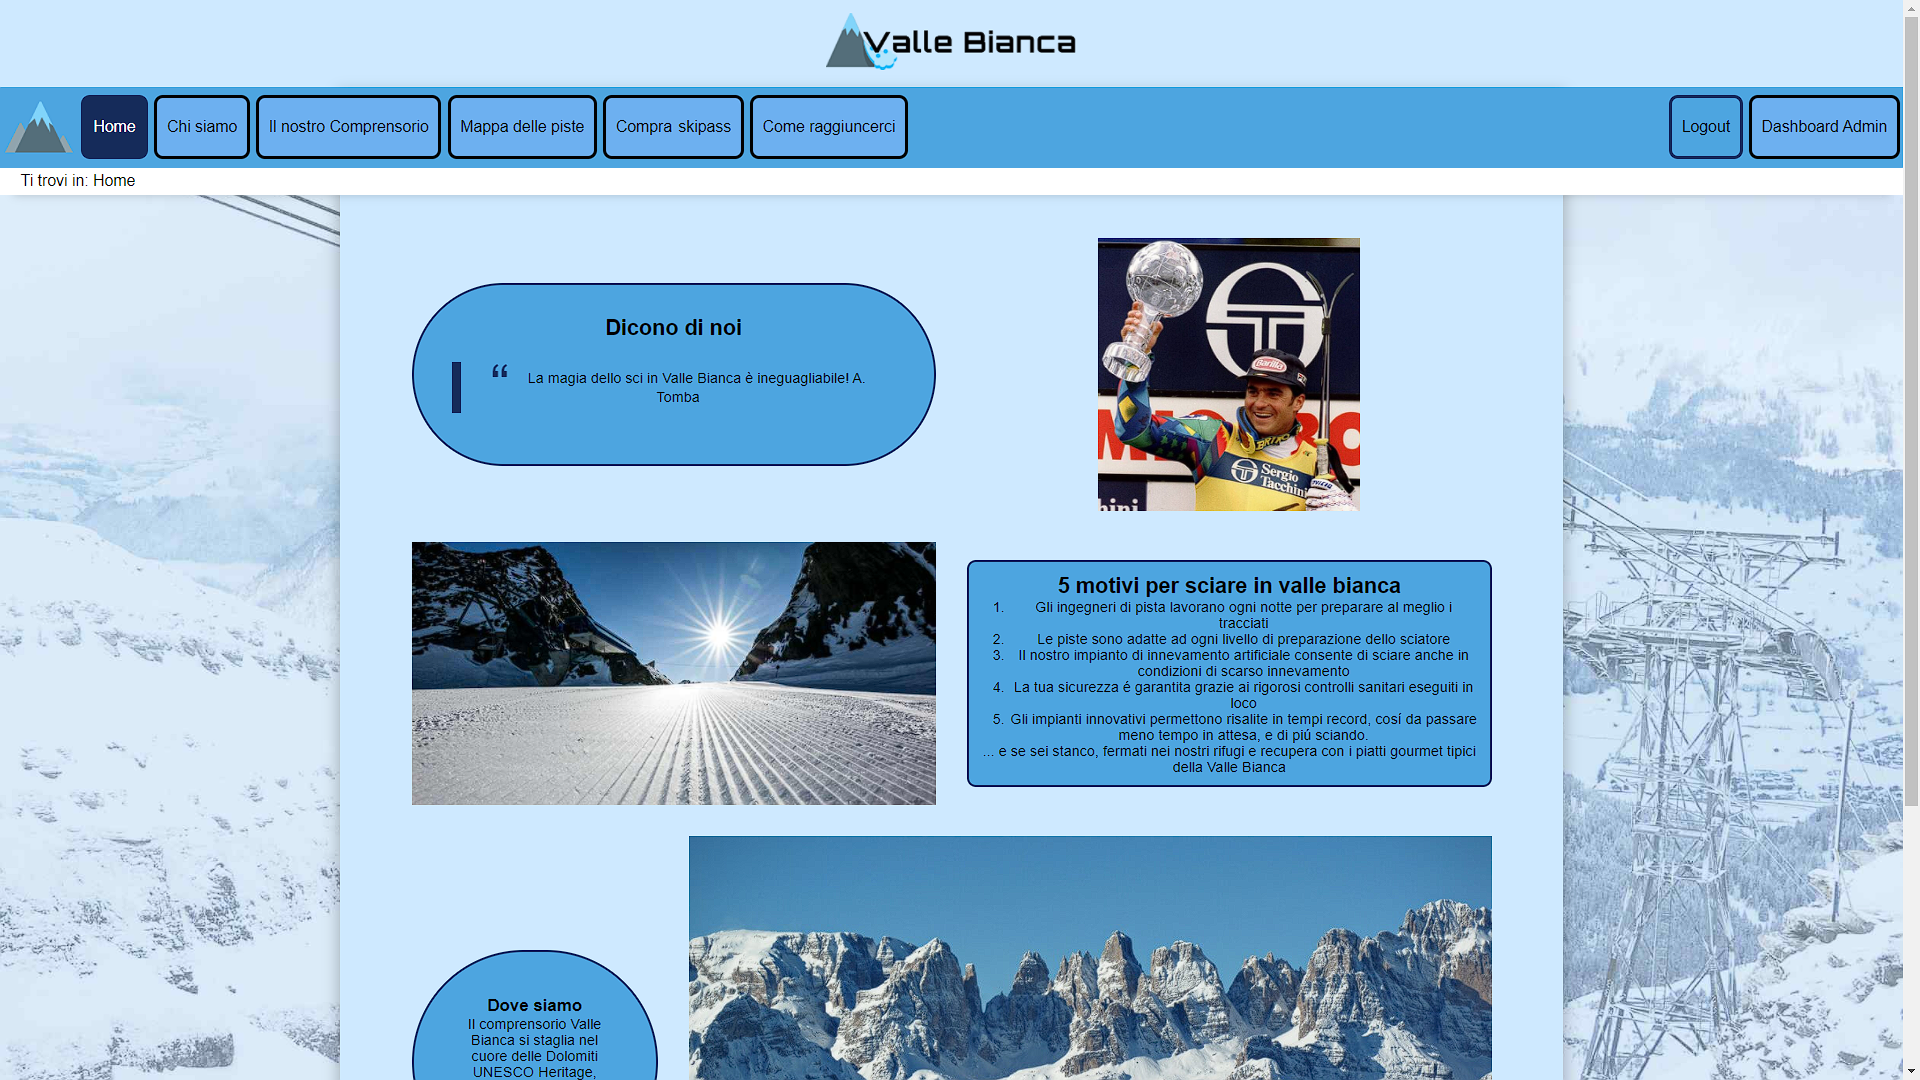
\includegraphics[width=0.8\textwidth]{desktop.png}
        \caption{Stile da desktop}
    \end{subfigure} 
    \begin{subfigure}{.4\textwidth}
        \centering
        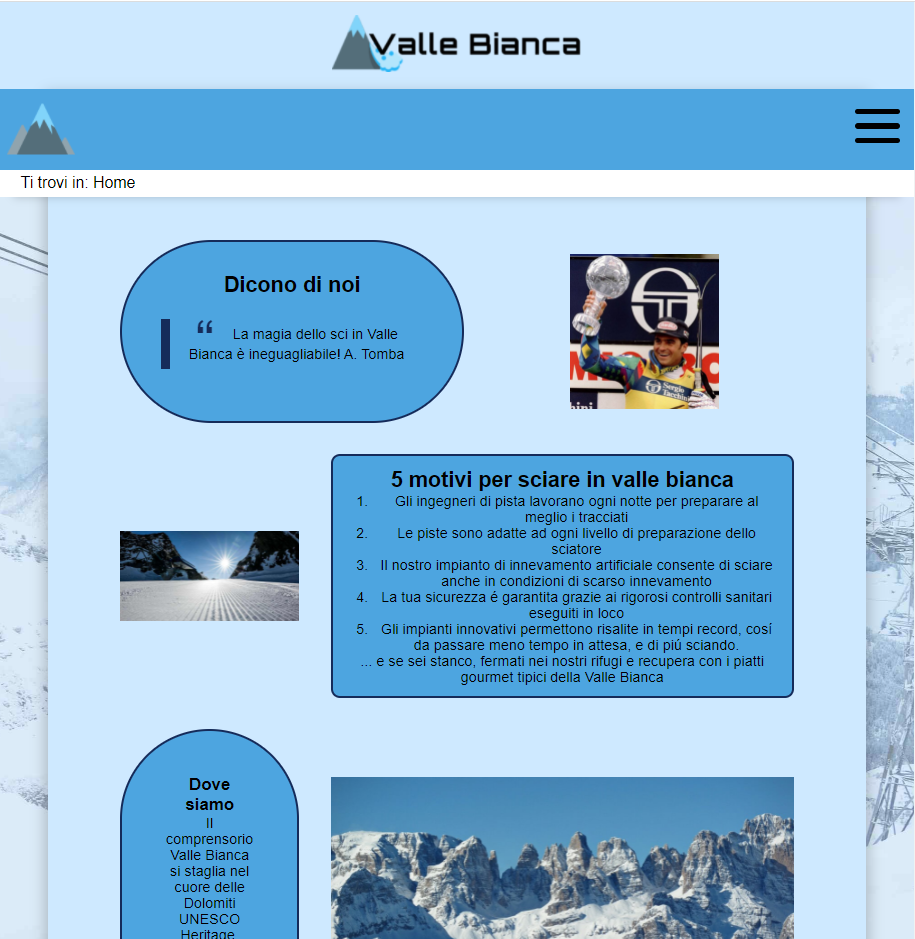
\includegraphics[width=0.8\textwidth]{tablet.png}
        \caption{Stile da tablet}
    \end{subfigure} 
    
\end{figure}

\subsubsection{Tablet}
Lo stile per i tablet, o in generale per dispositivi di medie dimensioni, si applica successivamente allo stile di base e modifica solamente il menu e la conformazione della pagina home.
Il menù diventa ad hamburger e si apre verticalmente per ridurre lo spazio occupato durante la navigazione.

\subsubsection{Cellulari}
Se visualizzato da smartphone il menù diventa invece un menù composto da icone posizionate sul fondo dello schermo in modo da renderli raggiungibili anche per chi utilizza il dispositivo con una sola mano.

Viene anche modificato il layout della homepage ed alcune tabelle vengono adattate per schermi più piccoli
\begin{figure}[h!]
    \begin{subfigure}{.45\textwidth}
        \centering
        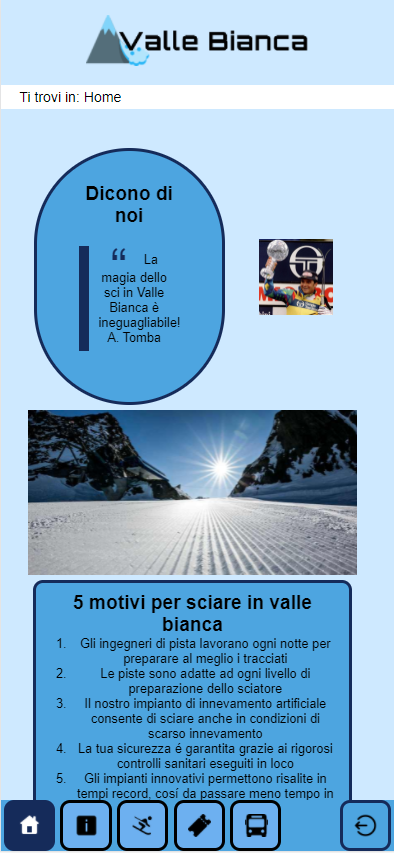
\includegraphics[width=.6\linewidth]{cellulare.png}
        \caption{Stile da cellulare}
    \end{subfigure} 
    \begin{subfigure}{.45\textwidth}
        \centering
        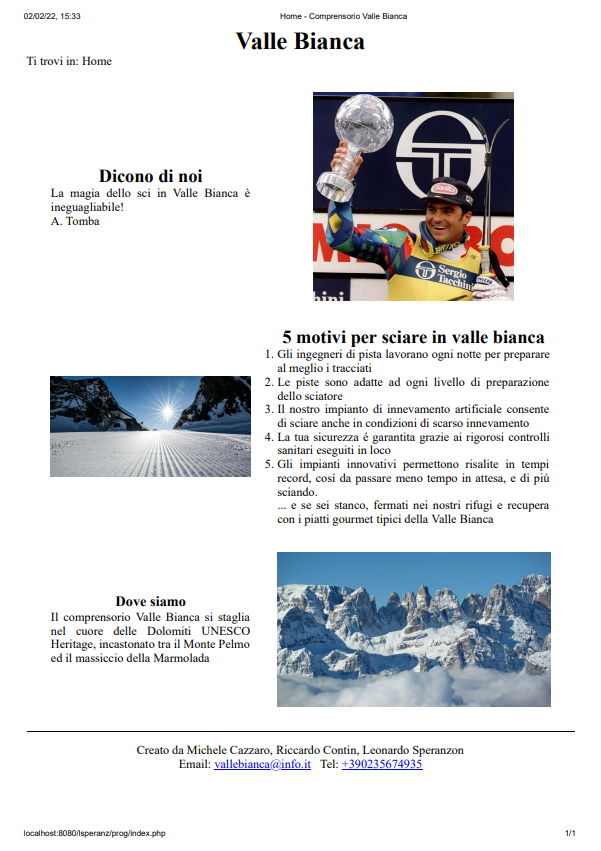
\includegraphics[width=.6\linewidth]{print.png}
        \caption{Stile per la stampa}
    \end{subfigure} 
\end{figure}

\subsubsection{Stampa}
Per la stampa delle pagine viene utilizzato un foglio di stile specifico che imposta un carattere più adatto alla lettura su carta e nasconde gli elementi superflui come il menu e gli aiuti alla navigazione.
La breadcrumb resta comunque visibile per dare maggiore contesto alla pagina una volta stampata.



Alcune pagine data la loro natura non sono state adattate per la stampa, queste pagine sono: shop, modificaComprensorio, modificaPrezzi e le pagine relative al processo di autenticazione.

\newpage
\subsection{Comportamento}

Per quanto riguarda l'utilizzo di JavaScript abbiamo cercato di implementare delle funzionalità che permettessero di rendere il sito migliore dal punto di vista funzionale ed estetico.
Questo però non va ad influire sull'utilizzo del sito, infatti nel caso in cui JavaScript non funzionasse o comunque non fosse disponibile il sito non perderebbe funzionalità, ma solo qualche dettaglio.

Le funzionalità implementate con JavaScript sono:
\begin{itemize}
    \item Permettere apertura e chiusura del menù da tablet premendo sul bottone menù;
    \item Permettere la comparsa e la scomparsa del bottone per tornare all'inizio della pagina in base alla posizione della pagina in cui ci troviamo;
    \item Controllo di username, password e email lato client;
    \item Ridimensionamento della map per poter mantenere i numeri dell'immagine presente nella pagina mappa come link alla pagina dettagli in caso di ridimensionamento dell'immagine, grazie ad uno script open source;
    \item Nascondere e mostrare i fieldset di interesse nella pagina modificaComprensorio;
    \item Nel form dello shop, validare i dati inseriti, funzionamento dei bottoni +/- e calcolo del prezzo totale in tempo reale.
\end{itemize}

Ovviamente tutto questo è separato dai contenuti in rispettivi file js contenuti nella cartella js per appunto mantenere una separazione fondamentale.

\subsection{PHP}

Oltre ai placeholder descritti precedentemente, l'utilizzo di PHP ci ha permesso diverse cose:
\begin{itemize}
    \item Collegamento al database che ci ha permesso di eseguire delle query di inserimento/eliminazione/modifica ma anche la possibilità
        di inserire nelle pagine i contenuti del database grazie ai segnaposti presenti nei file html;
    \item Controllo delle sessioni per distinguere i privilegi tra gli utenti;
    \item Controllare dati inseriti e gestione degli errori lato server.
\end{itemize}

I file PHP sono stati divisi:
\begin{itemize}
    \item File che visualizzano i contenuti includendo i file html direttamente nella radice;
    \item File di utilità dentro la cartella php\textunderscore vari.
\end{itemize}